% Important: If latex complains about unicode characters,
% please use "\usepackage[utf8x]{inputenc}" in your preamble
% You can change the size of the picture by putting it into the construct:
% 1) \resizebox{10cm}{!}{"below picture"} to scale horizontally to 10 cm
% 2) \resizebox{!}{15cm}{"below picture"} to scale vertically to 15 cm
% 3) \resizebox{10cm}{15cm}{"below picture"} a combination of above two
% It is not recomended to use the scale option of the tikzpicture environment.
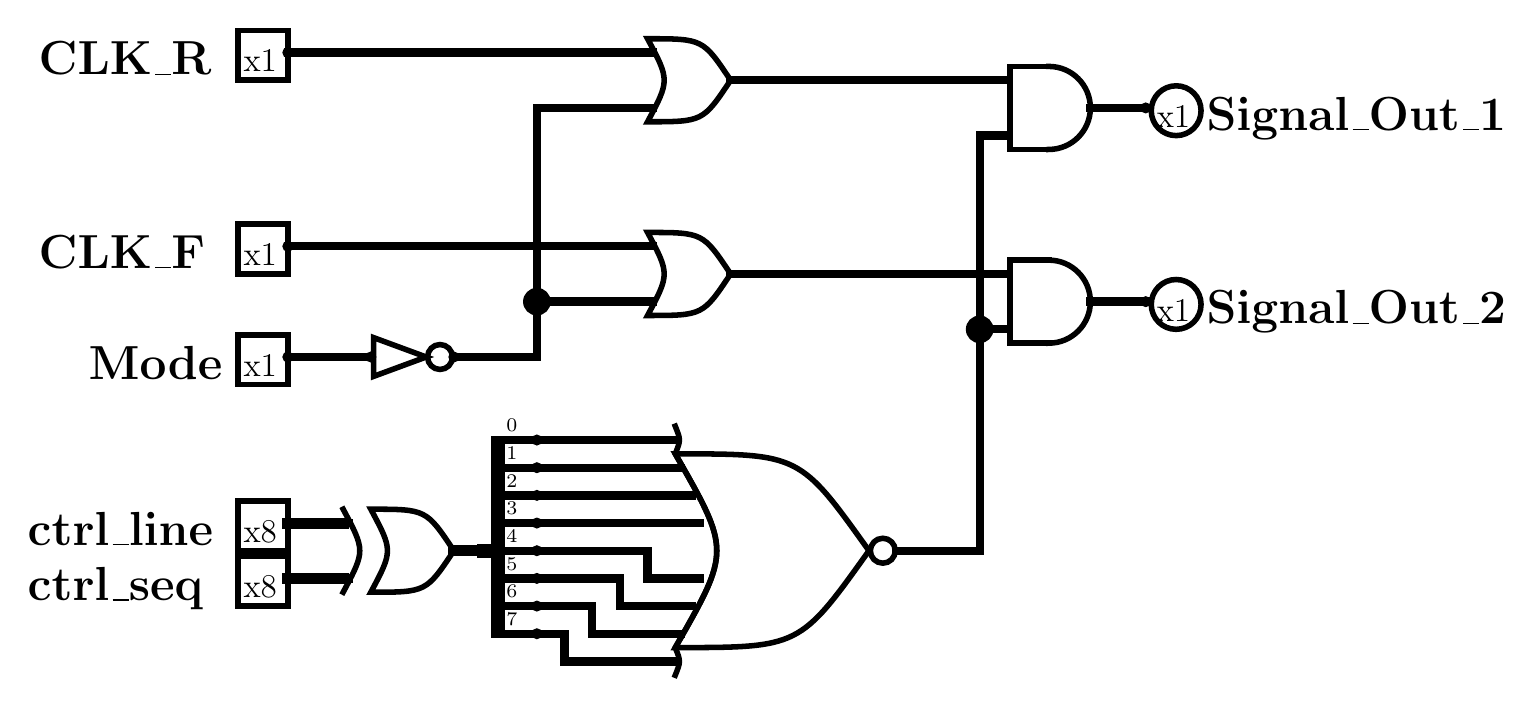
\begin{tikzpicture}[x=1pt,y=-1pt,line cap=rect]
\def\logisimfontA#1{\fontfamily{cmr}{#1}} % Replaced by logisim, original font was "SansSerif"
\definecolor{custcol_0_0_0}{RGB}{0, 0, 0}
\definecolor{custcol_ff_ff_ff}{RGB}{255, 255, 255}
\draw [line width=3.0pt, custcol_0_0_0 ]  (248.0,95.0) -- (348.0,95.0) ;
\draw [line width=3.0pt, custcol_0_0_0 ]  (248.0,25.0) -- (348.0,25.0) ;
\draw [line width=3.0pt, custcol_0_0_0 ]  (88.0,125.0) -- (118.0,125.0) ;
\draw [line width=3.0pt, custcol_0_0_0 ]  (378.0,105.0) -- (398.0,105.0) ;
\draw [line width=3.0pt, custcol_0_0_0 ]  (378.0,35.0) -- (398.0,35.0) ;
\draw [line width=4.0pt, custcol_0_0_0 ]  (88.0,185.0) -- (108.0,185.0) ;
\draw [line width=4.0pt, custcol_0_0_0 ]  (88.0,205.0) -- (108.0,205.0) ;
\draw [line width=3.0pt, custcol_0_0_0 ]  (338.0,115.0) -- (348.0,115.0) ;
\draw [line width=3.0pt, custcol_0_0_0 ]  (308.0,195.0) -- (338.0,195.0) -- (338.0,115.0) -- (338.0,45.0) -- (348.0,45.0) ;
\draw [line width=4.0pt, custcol_0_0_0 ]  (148.0,195.0) -- (158.0,195.0) ;
\fill [line width=3.0pt, custcol_0_0_0]  (338.0,115.0) ellipse (5.0 and 5.0 );
\fill [line width=3.0pt, custcol_0_0_0]  (178.0,105.0) ellipse (5.0 and 5.0 );
\draw [line width=2.0pt, custcol_0_0_0 ]  (70.0,77.0) -- (87.0,77.0) ;
\draw [line width=2.0pt, custcol_0_0_0 ]  (88.0,77.0) -- (88.0,94.0) ;
\draw [line width=2.0pt, custcol_0_0_0 ]  (88.0,95.0) -- (71.0,95.0) ;
\draw [line width=2.0pt, custcol_0_0_0 ]  (70.0,95.0) -- (70.0,78.0) ;
\logisimfontA{\fontsize{12pt}{12pt}\selectfont\node[inner sep=0, outer sep=0, custcol_0_0_0, anchor=base west] at  (72.0,92.0)  {x1};}
\logisimfontA{\fontsize{16pt}{16pt}\fontseries{bx}\selectfont\node[inner sep=0, outer sep=0, custcol_0_0_0, anchor=base west] at  (-2.0,93.0)  {CLK\_F};}
\fill [line width=2.0pt, custcol_0_0_0]  (88.0,85.0) ellipse (2.0 and 2.0 );
\draw [line width=2.0pt, custcol_0_0_0 ]  (70.0,117.0) -- (87.0,117.0) ;
\draw [line width=2.0pt, custcol_0_0_0 ]  (88.0,117.0) -- (88.0,134.0) ;
\draw [line width=2.0pt, custcol_0_0_0 ]  (88.0,135.0) -- (71.0,135.0) ;
\draw [line width=2.0pt, custcol_0_0_0 ]  (70.0,135.0) -- (70.0,118.0) ;
\logisimfontA{\fontsize{12pt}{12pt}\selectfont\node[inner sep=0, outer sep=0, custcol_0_0_0, anchor=base west] at  (72.0,132.0)  {x1};}
\logisimfontA{\fontsize{16pt}{16pt}\fontseries{bx}\selectfont\node[inner sep=0, outer sep=0, custcol_0_0_0, anchor=base west] at  (16.0,133.0)  {Mode};}
\fill [line width=2.0pt, custcol_0_0_0]  (88.0,125.0) ellipse (2.0 and 2.0 );
\draw [line width=2.0pt, custcol_0_0_0 ]  (70.0,177.0) -- (87.0,177.0) ;
\draw [line width=2.0pt, custcol_0_0_0 ]  (88.0,177.0) -- (88.0,194.0) ;
\draw [line width=2.0pt, custcol_0_0_0 ]  (88.0,195.0) -- (71.0,195.0) ;
\draw [line width=2.0pt, custcol_0_0_0 ]  (70.0,195.0) -- (70.0,178.0) ;
\logisimfontA{\fontsize{12pt}{12pt}\selectfont\node[inner sep=0, outer sep=0, custcol_0_0_0, anchor=base west] at  (72.0,192.0)  {x8};}
\logisimfontA{\fontsize{16pt}{16pt}\fontseries{bx}\selectfont\node[inner sep=0, outer sep=0, custcol_0_0_0, anchor=base west] at  (-6.0,193.0)  {ctrl\_line};}
\fill [line width=2.0pt, custcol_0_0_0]  (88.0,185.0) ellipse (2.0 and 2.0 );
\draw [line width=2.0pt, custcol_0_0_0 ]  (70.0,197.0) -- (87.0,197.0) ;
\draw [line width=2.0pt, custcol_0_0_0 ]  (88.0,197.0) -- (88.0,214.0) ;
\draw [line width=2.0pt, custcol_0_0_0 ]  (88.0,215.0) -- (71.0,215.0) ;
\draw [line width=2.0pt, custcol_0_0_0 ]  (70.0,215.0) -- (70.0,198.0) ;
\logisimfontA{\fontsize{12pt}{12pt}\selectfont\node[inner sep=0, outer sep=0, custcol_0_0_0, anchor=base west] at  (72.0,212.0)  {x8};}
\logisimfontA{\fontsize{16pt}{16pt}\fontseries{bx}\selectfont\node[inner sep=0, outer sep=0, custcol_0_0_0, anchor=base west] at  (-6.0,213.0)  {ctrl\_seq};}
\fill [line width=2.0pt, custcol_0_0_0]  (88.0,205.0) ellipse (2.0 and 2.0 );
\draw [line width=2.0pt, custcol_0_0_0 ]  (70.0,7.0) -- (87.0,7.0) ;
\draw [line width=2.0pt, custcol_0_0_0 ]  (88.0,7.0) -- (88.0,24.0) ;
\draw [line width=2.0pt, custcol_0_0_0 ]  (88.0,25.0) -- (71.0,25.0) ;
\draw [line width=2.0pt, custcol_0_0_0 ]  (70.0,25.0) -- (70.0,8.0) ;
\logisimfontA{\fontsize{12pt}{12pt}\selectfont\node[inner sep=0, outer sep=0, custcol_0_0_0, anchor=base west] at  (72.0,22.0)  {x1};}
\logisimfontA{\fontsize{16pt}{16pt}\fontseries{bx}\selectfont\node[inner sep=0, outer sep=0, custcol_0_0_0, anchor=base west] at  (-2.0,23.0)  {CLK\_R};}
\fill [line width=2.0pt, custcol_0_0_0]  (88.0,15.0) ellipse (2.0 and 2.0 );
\draw [line width=3.0pt, custcol_0_0_0 ]  (228.0,155.0) -- (178.0,155.0) -- (164.0,155.0) ;
\draw [line width=3.0pt, custcol_0_0_0 ]  (228.0,235.0) -- (188.0,235.0) -- (188.0,225.0) -- (178.0,225.0) -- (164.0,225.0) ;
\draw [line width=5.0pt, custcol_0_0_0 ]  (159.0,195.0) -- (164.0,195.0) ;
\draw [line width=5.0pt, custcol_0_0_0 ]  (164.0,156.0) -- (164.0,224.0) ;
\logisimfontA{\fontsize{7pt}{7pt}\selectfont\node[inner sep=0, outer sep=0, custcol_0_0_0, anchor=base west] at  (167.0,152.0)  {0};}
\logisimfontA{\fontsize{7pt}{7pt}\selectfont\node[inner sep=0, outer sep=0, custcol_0_0_0, anchor=base west] at  (167.0,162.0)  {1};}
\logisimfontA{\fontsize{7pt}{7pt}\selectfont\node[inner sep=0, outer sep=0, custcol_0_0_0, anchor=base west] at  (167.0,172.0)  {2};}
\logisimfontA{\fontsize{7pt}{7pt}\selectfont\node[inner sep=0, outer sep=0, custcol_0_0_0, anchor=base west] at  (167.0,182.0)  {3};}
\logisimfontA{\fontsize{7pt}{7pt}\selectfont\node[inner sep=0, outer sep=0, custcol_0_0_0, anchor=base west] at  (167.0,192.0)  {4};}
\logisimfontA{\fontsize{7pt}{7pt}\selectfont\node[inner sep=0, outer sep=0, custcol_0_0_0, anchor=base west] at  (167.0,202.0)  {5};}
\logisimfontA{\fontsize{7pt}{7pt}\selectfont\node[inner sep=0, outer sep=0, custcol_0_0_0, anchor=base west] at  (167.0,212.0)  {6};}
\logisimfontA{\fontsize{7pt}{7pt}\selectfont\node[inner sep=0, outer sep=0, custcol_0_0_0, anchor=base west] at  (167.0,222.0)  {7};}
\fill [line width=5.0pt, custcol_0_0_0]  (158.0,195.0) ellipse (2.0 and 2.0 );
\fill [line width=5.0pt, custcol_0_0_0]  (178.0,155.0) ellipse (2.0 and 2.0 );
\fill [line width=5.0pt, custcol_0_0_0]  (178.0,165.0) ellipse (2.0 and 2.0 );
\fill [line width=5.0pt, custcol_0_0_0]  (178.0,175.0) ellipse (2.0 and 2.0 );
\fill [line width=5.0pt, custcol_0_0_0]  (178.0,185.0) ellipse (2.0 and 2.0 );
\fill [line width=5.0pt, custcol_0_0_0]  (178.0,195.0) ellipse (2.0 and 2.0 );
\fill [line width=5.0pt, custcol_0_0_0]  (178.0,205.0) ellipse (2.0 and 2.0 );
\fill [line width=5.0pt, custcol_0_0_0]  (178.0,215.0) ellipse (2.0 and 2.0 );
\fill [line width=5.0pt, custcol_0_0_0]  (178.0,225.0) ellipse (2.0 and 2.0 );
\draw [line width=2.0pt, custcol_0_0_0]  (409.0,106.0) ellipse (9.0 and 9.0 );
\logisimfontA{\fontsize{12pt}{12pt}\selectfont\node[inner sep=0, outer sep=0, custcol_0_0_0, anchor=base west] at  (402.0,112.0)  {x1};}
\logisimfontA{\fontsize{16pt}{16pt}\fontseries{bx}\selectfont\node[inner sep=0, outer sep=0, custcol_0_0_0, anchor=base west] at  (420.0,113.0)  {Signal\_Out\_2};}
\fill [line width=2.0pt, custcol_0_0_0]  (398.0,105.0) ellipse (2.0 and 2.0 );
\draw [line width=2.0pt, custcol_0_0_0]  (409.0,36.0) ellipse (9.0 and 9.0 );
\logisimfontA{\fontsize{12pt}{12pt}\selectfont\node[inner sep=0, outer sep=0, custcol_0_0_0, anchor=base west] at  (402.0,42.0)  {x1};}
\logisimfontA{\fontsize{16pt}{16pt}\fontseries{bx}\selectfont\node[inner sep=0, outer sep=0, custcol_0_0_0, anchor=base west] at  (420.0,43.0)  {Signal\_Out\_1};}
\fill [line width=2.0pt, custcol_0_0_0]  (398.0,35.0) ellipse (2.0 and 2.0 );
\draw [line width=2.0pt, custcol_0_0_0 ]  (138.0,125.0) -- (119.0,118.0) -- (119.0,132.0) -- cycle;
\draw [line width=2.0pt, custcol_0_0_0]  (143.0,125.0) ellipse (4.5 and 4.5 );
\fill [line width=2.0pt, custcol_0_0_0]  (148.0,125.0) ellipse (2.0 and 2.0 );
\fill [line width=2.0pt, custcol_0_0_0]  (118.0,125.0) ellipse (2.0 and 2.0 );
\draw [line width=3.0pt, custcol_0_0_0 ]  (108.0,185.0) -- (110.0,185.0) ;
\draw [line width=3.0pt, custcol_0_0_0 ]  (108.0,205.0) -- (110.0,205.0) ;
\draw [line width=2.0pt, custcol_0_0_0 ]  (148.0,195.0) .. controls  (138.0,180.0)  ..  (118.0,180.0) .. controls  (126.0,195.0)  ..  (118.0,210.0) .. controls  (138.0,210.0)  ..  (148.0,195.0) -- cycle ;
\draw [line width=2.0pt, custcol_0_0_0 ]  (108.0,180.0) .. controls  (116.0,195.0)  ..  (108.0,210.0) ;
\draw [line width=3.0pt, custcol_0_0_0 ]  (88.0,85.0) -- (218.0,85.0) -- (220.0,85.0) ;
\draw [line width=3.0pt, custcol_0_0_0 ]  (178.0,105.0) -- (218.0,105.0) -- (220.0,105.0) ;
\draw [line width=2.0pt, custcol_0_0_0 ]  (248.0,95.0) .. controls  (238.0,80.0)  ..  (218.0,80.0) .. controls  (226.0,95.0)  ..  (218.0,110.0) .. controls  (238.0,110.0)  ..  (248.0,95.0) -- cycle ;
\draw [line width=3.0pt, custcol_0_0_0 ]  (88.0,15.0) -- (218.0,15.0) -- (220.0,15.0) ;
\draw [line width=3.0pt, custcol_0_0_0 ]  (148.0,125.0) -- (178.0,125.0) -- (178.0,105.0) -- (178.0,35.0) -- (218.0,35.0) -- (220.0,35.0) ;
\draw [line width=2.0pt, custcol_0_0_0 ]  (248.0,25.0) .. controls  (238.0,10.0)  ..  (218.0,10.0) .. controls  (226.0,25.0)  ..  (218.0,40.0) .. controls  (238.0,40.0)  ..  (248.0,25.0) -- cycle ;
\draw [line width=3.0pt, custcol_0_0_0 ]  (164.0,165.0) -- (178.0,165.0) -- (228.0,165.0) -- (230.0,165.0) ;
\draw [line width=3.0pt, custcol_0_0_0 ]  (164.0,175.0) -- (178.0,175.0) -- (228.0,175.0) -- (234.0,175.0) ;
\draw [line width=3.0pt, custcol_0_0_0 ]  (164.0,185.0) -- (178.0,185.0) -- (228.0,185.0) -- (237.0,185.0) ;
\draw [line width=3.0pt, custcol_0_0_0 ]  (164.0,195.0) -- (178.0,195.0) -- (218.0,195.0) -- (218.0,205.0) -- (228.0,205.0) -- (237.0,205.0) ;
\draw [line width=3.0pt, custcol_0_0_0 ]  (164.0,205.0) -- (178.0,205.0) -- (208.0,205.0) -- (208.0,215.0) -- (228.0,215.0) -- (234.0,215.0) ;
\draw [line width=3.0pt, custcol_0_0_0 ]  (164.0,215.0) -- (178.0,215.0) -- (198.0,215.0) -- (198.0,225.0) -- (228.0,225.0) -- (230.0,225.0) ;
\draw [line width=2.0pt, custcol_0_0_0 ]  (298.0,195.0) .. controls  (273.0,160.0)  ..  (228.0,160.0) .. controls  (248.0,195.0)  ..  (228.0,230.0) .. controls  (273.0,230.0)  ..  (298.0,195.0) -- cycle ;
\draw [line width=2.0pt, custcol_0_0_0 ]  (228.0,150.0) .. controls  (230.0,155.0)  ..  (228.0,160.0) .. controls  (248.0,195.0)  ..  (228.0,230.0) .. controls  (230.0,235.0)  ..  (228.0,240.0) ;
\draw [line width=2.0pt, custcol_0_0_0]  (303.0,195.0) ellipse (4.5 and 4.5 );
\draw [line width=2.0pt, custcol_0_0_0] (363.0,120.0) arc (90.0:-90.0:15.0 and 15.0 );
\draw [line width=2.0pt, custcol_0_0_0 ]  (363.0,90.0) -- (349.0,90.0) -- (349.0,120.0) -- (363.0,120.0) ;
\draw [line width=2.0pt, custcol_0_0_0] (363.0,50.0) arc (90.0:-90.0:15.0 and 15.0 );
\draw [line width=2.0pt, custcol_0_0_0 ]  (363.0,20.0) -- (349.0,20.0) -- (349.0,50.0) -- (363.0,50.0) ;
\end{tikzpicture}

